\documentclass[UTF8,a4paper,10pt,fontset=fandol]{ctexart}
\usepackage[margin=23mm]{geometry}
\usepackage{amsmath,amssymb,graphicx,booktabs,tabularx,array,adjustbox}
\usepackage{xcolor}
\usepackage[colorlinks=true,linkcolor=black,urlcolor=blue!45!black]{hyperref}
\setlength{\parindent}{2em}
\setlength{\parskip}{0.3em}
\linespread{1.16}
\setlength{\emergencystretch}{2em}
\setlength{\tabcolsep}{3pt}
\renewcommand{\arraystretch}{1.3}
\title{联邦长尾学习中的尾部类别知识保持\\与跨客户端知识迁移}
\author{}
\date{}
\begin{document}
\maketitle
\vspace{-2em}


\section*{摘要}

联邦长尾学习中，尾部类别的学习条件同时取决于样本数量及其在客户端之间的分布。当稀缺样本集中于少数客户端时，全局模型在训练中已经获得的分类能力，可能随后续协同更新逐渐下降。本文通过 Client-LT 划分研究这一知识保持问题：在保持全局长尾样本池不变的条件下，将尾部类别样本集中分配给同一组少数客户端，并比较不同训练策略下的尾部类别表现。客户端更新分析进一步显示，持有目标类别样本的客户端与能够改善该类别预测的客户端并不完全重合，这为利用更广泛的客户端更新提供了依据。基于这些观察，我们提出来源感知的协同适配框架。首先，根据客户端类别分布确定聚合权重；随后，以客户端更新对预测间隔的影响衡量有效支持的集中程度，结合当前改善方向与历史预测间隔构造知识保持目标；同时，利用客户端反馈学习已有更新的低维矩阵组合，为全局模型提供补充更新。在 CIFAR-100-LT 的 Client-LT 开发实验中，完整配置的尾部类别准确率与整体准确率分别达到 72.63\% 和 70.47\%。两个随机种子的模块实验及同起点继续训练分析表明，来源感知权重和历史目标有助于保持尾部类别能力，并呈现出知识保持与继续学习之间的性能取舍。


\section*{1. 引言}

联邦视觉分类通过多个客户端的本地训练与模型聚合，学习一个共同使用的全局模型 [1]。对于尾部类别，其学习条件不仅取决于系统中共有多少样本，也取决于这些样本分布在哪里。以多工厂联合质检为例，若某种罕见缺陷与特定设备或工艺有关，它的样本可能集中在少数工厂。联合训练需要将这些有限样本所提供的识别能力融入全局模型，并在其他工厂持续参与训练时保留这种能力。视觉语言模型提供的可迁移表示 [2] 为稀缺类别学习带来了有利起点，也使一个问题更加具体：当模型已经能够识别部分尾部类别样本时，后续联邦训练如何延续并改善这一能力？


已有研究从适配强度、类别感知和知识保持等角度改善长尾学习。LIFT 发现重度微调可能损伤基础模型的尾部类别表现，并采用轻量适配 [3]；CAPT 通过类别感知提示处理联邦数据异质性与类别不平衡 [4]；FedPuReL 利用零样本预测引导全局知识保持，并进一步开展个性化残差学习 [5]。与此同时，FedNTD 将跨轮知识遗忘与联邦数据异质性联系起来，通过蒸馏维护全局知识 [6]。这些研究说明，适配过程需要兼顾新数据的学习与已有能力的保持。本文进一步考察尾部类别样本的客户端分布，以及这种分布下全局模型分类能力的演变。


我们用 Client-LT 划分描述尾部类别样本共同集中于少数客户端的情形，并跟踪相同全局样本池下的完整训练过程。实验显示，尾部类别准确率能够在训练中达到较高水平，随后出现回落；回落幅度同时随客户端分配和参数更新策略变化。固定每类样本总量与每个客户端样本总量的配对分析，也观察到了不同分配下的保持差异。这使研究目标落在一个具体问题上：在保持数据原有归属、继续训练同一个全局模型的条件下，如何维护少数有效来源所支撑的类别能力，并利用其他客户端更新进一步改善尾部类别学习？


实现这一目标需要同时处理知识保持与跨客户端更新利用。对于知识保持，类别频率和标签所在位置只能描述数据分布，方法还需要判断当前哪些更新能够改善预测，以及此前已经获得哪些值得保留的改善。客户端更新分析发现，不含目标类别样本的客户端也会对该类别产生正向作用，因此有效支持需要依据更新的实际影响来识别。对于跨客户端更新利用，不同更新的作用具有类别依赖性，普通参数平均之外还存在根据目标类别反馈重新组合更新的空间。LoRA 因子冻结与交替优化分别提供了限制参数变化和保留适配能力的途径 [7, 8]；本文在允许因子继续适应的基础上，将本地类别反馈用于指导知识保持与更新组合。


为此，我们提出来源感知的协同适配框架，将类别分布感知聚合、知识保持和跨客户端知识迁移连接起来。聚合阶段通过 joint 权重协调客户端类别分布在全局更新中的体现。知识保持阶段根据各客户端更新对预测间隔的正向影响，识别有效支持较集中的客户端—类别组合，并结合当前预测间隔和历史记录确定保持目标；随后在常规更新附近修正模型，同时考虑分类训练损失。知识迁移阶段以已有客户端更新为基础，通过本地尾部与非尾部类别反馈学习低维组合矩阵，形成一个共享补充更新。这样，少数客户端提供的类别信息既参与当前训练，也通过历史目标持续影响后续适配，而其他客户端更新则获得面向这些类别进一步调整的机会。


本文的贡献体现在三个方面。首先，我们以类别样本数量和客户端分布两个维度组织 Client-LT 分析，通过训练轨迹与固定边际对照刻画尾部类别的保持问题，并考察不同客户端更新的正向支持。其次，我们提出来源感知的知识保持方法，将有效支持的集中程度、当前改善目标和历史预测间隔共同用于约束全局模型的适配。最后，我们将该方法与类别分布感知聚合及反馈驱动的更新组合构成完整框架，通过分类性能、两个随机种子的模块消融和样本预测变化分析，呈现尾部类别收益及其与其他类别性能的关系。


\section*{2. 相关工作}

\subsection*{2.1 联邦长尾学习与视觉基础模型适配}

类别不平衡使训练目标更多地受到高频类别影响。Logit adjustment 从类别频率出发修正分类目标，为长尾分类提供了直接的损失设计 [9]。在联邦场景中，FedLF 结合自适应 logit 调整与特征优化 [10]，FedYoYo 通过增强视图之间的自蒸馏和分布感知 logit 调整改善本地表示 [11]，FedReLa 从样本重标记的角度处理类别不平衡与客户端异质性 [12]。这些方法围绕数据、表示和分类目标开展调整。本文进一步引入训练轨迹上的保持目标，使已经获得的类别判别能力参与后续更新的优化。


视觉语言模型为这一问题提供了具有迁移能力的初始化。LIFT 研究微调强度对长尾性能的影响 [3]，CAPT 将类别感知提示用于联邦长尾学习 [4]，FedPuReL 将基础模型的类别平衡性保持与个性化学习结合 [5]。本文关注固定类别集合下的单一全局模型，并使用训练过程中逐步登记的历史预测间隔作为保持参照。这一参照随模型获得持续改善而更新，使保持对象覆盖适配过程中形成的分类能力。


\subsection*{2.2 知识保持与联邦低秩适配}

训练中分类正确的样本随后转为错误，反映了样本层面的能力丢失。Toneva 等通过此类遗忘事件研究单一分类任务的学习动态 [13]；FedNTD 则在联邦学习中利用非真类蒸馏维护全局知识 [6]。本文以本地客户端—类别组合的预测间隔构造保持目标，并根据有效支持来源的集中程度分配保持权重。历史记录为目标提供时间参照，来源响应为约束提供差异化权重，两者共同决定当前更新应优先维护哪些分类能力。


LoRA 用低秩参数增量实现预训练模型适配 [14]，其两个因子的训练方式也影响联邦优化。FFA-LoRA 固定随机初始化的因子，仅训练另一因子 [7]；RoLoRA 采用交替优化 [8]；FedSVD 通过全局 SVD 重参数化调整低秩因子 [15]；LoRA-A$^2$ 结合交替冻结与自适应秩选择 [16]。本文采用分阶段因子训练，并在常规适配结果上加入类别功能约束：参数更新由本地分类任务产生，更新后的预测间隔则决定进一步修正的方向。


\subsection*{2.3 客户端贡献评估与更新协调}

不同客户端更新之间的关系为聚合设计提供了信息。FedFV 根据梯度冲突协调客户端更新 [17]，ShapFed 评估类别相关的客户端贡献并据此进行加权聚合 [18]，FedFomo 根据客户端从其他模型获得的收益学习个性化组合 [19]。本文将客户端更新的作用用于两个具体环节：在知识保持中，以正向响应的集中程度确定保持优先级；在知识迁移中，用客户端反馈优化每个来源、每个 LoRA 层的矩阵变换，将已有更新组合为一个加入全局模型的共享残差。


\section*{3. 问题定义与动机观察}

\subsection*{3.1 类别样本数量与客户端分布}

考虑由 $K$ 个客户端共同训练的 $C$ 类视觉分类任务。客户端 $k$ 保存本地数据集，系统在整个训练期间使用固定类别集合，并在每轮更新后评估同一个全局模型。记客户端 $k$ 中类别 $c$ 的样本数为 $n_{kc}$，则


\begin{center}\begin{adjustbox}{max width=\linewidth}$\displaystyle n_c=\sum_{k=1}^{K}n_{kc},\qquad
n_k=\sum_{c=1}^{C}n_{kc},\qquad
n_{kc}=n_c\,p(k\mid c).$\end{adjustbox}\end{center}

其中，$n_c$ 描述类别样本数量，$p(k\mid c)$ 描述该类别样本在客户端之间的分布。本文通过全局长尾程度 $\mathrm{IF}=n_{\max}/n_{\min}$ 和客户端集中程度 $\lambda_T$ 分别控制这两个维度。


Client-LT 预先选取占比为 $q_T$ 的客户端组，将比例约为 $q_T+(1-q_T)\lambda_T$ 的尾部类别样本分配给该组，再在组内和组外分别进行 Dirichlet 分配。随着 $\lambda_T$ 增大，多个尾部类别的样本共同向这一客户端组集中。实验中的 $q_T=0.1$、$\lambda_T=0.75$ 对应约 77.5\% 的目标分配比例。由于组外仍有尾部类别样本，后续反馈由所有实际持有相应样本的客户端提供。


图 1 展示基于 CIFAR-100 [20] 构建的长尾样本池在客户端之间的实际分配。两个划分使用相同的 10,847 张训练图像，其中尾部 20 类共 153 张图像。Client-LT 中，尾部样本最多的 3 个客户端持有其中 119 张，比例为 77.78\%；常规逐类 Dirichlet 划分中，该比例为 19.61\%。在 Client-LT 中，这 3 个客户端的全部训练样本合计仅占全局样本量的约 1.20\%。因此，描述某组客户端在尾部类别上的重要性，需要同时考察其类别组成和总数据量。


\begin{center}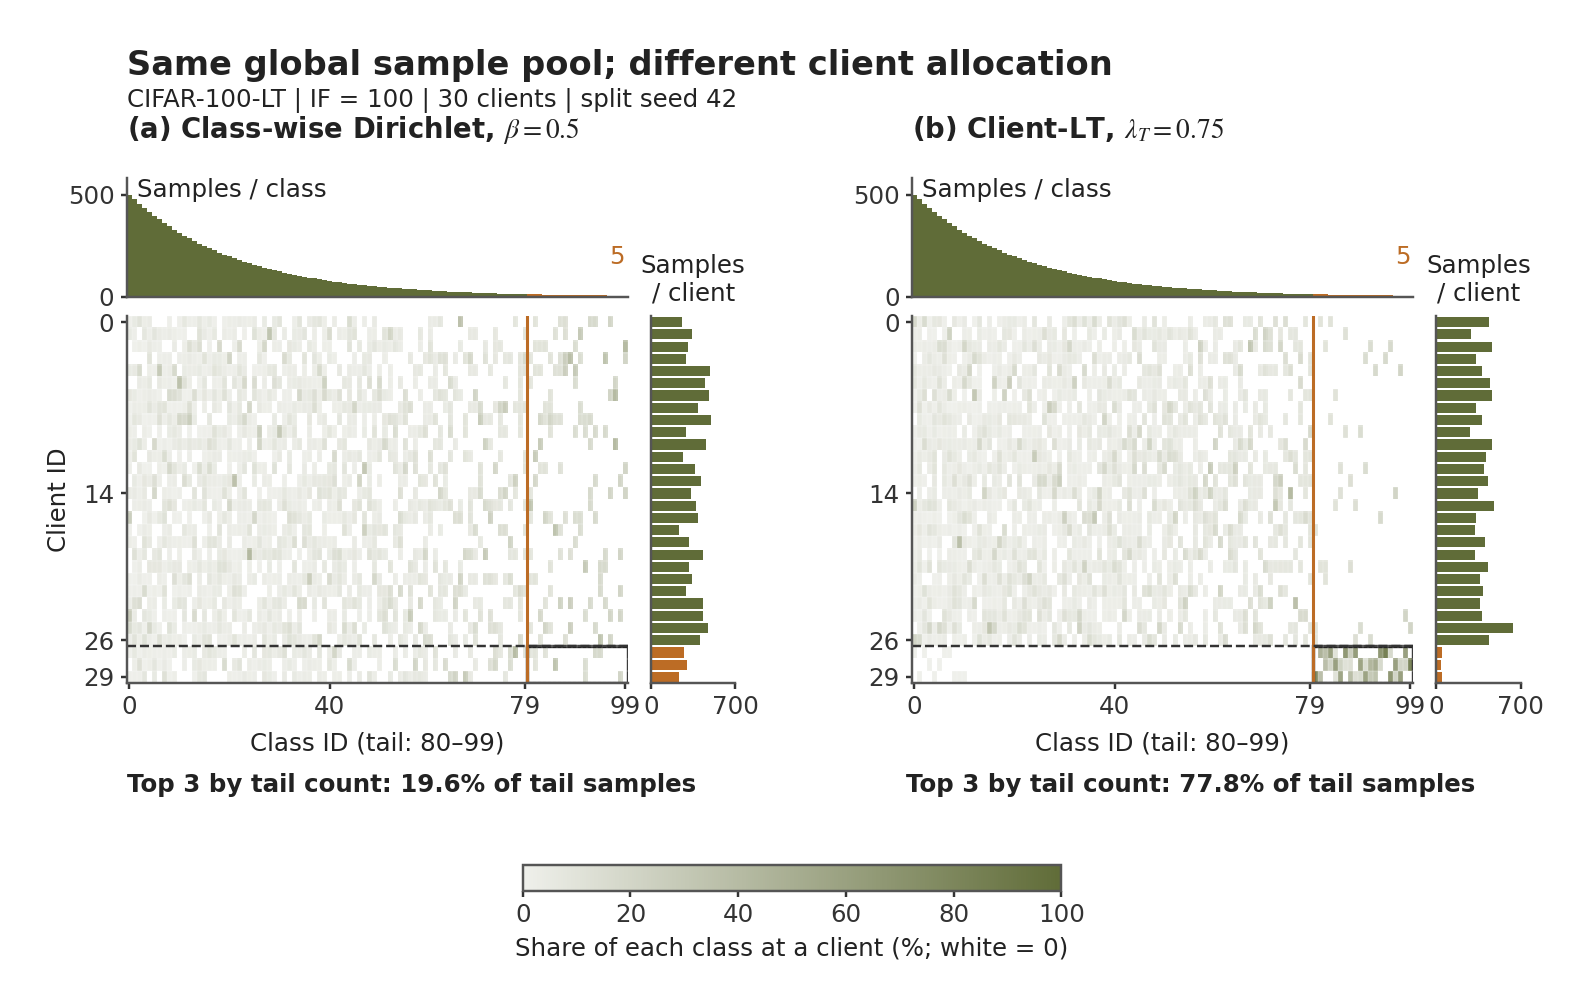
\includegraphics[width=0.95\linewidth]{partition_comparison.png}\end{center}

{\small\noindent 图 1. 相同全局长尾样本池下的客户端分配。热图按类别归一化，上方和右方柱图分别表示类别样本数与客户端样本数。Client-LT 将大部分尾部类别样本共同分配给少数客户端。\par}

\subsection*{3.2 尾部类别能力随训练过程发生回落}

我们首先比较相同全局长尾样本池下的训练轨迹。模型采用 CLIP ViT-B/16 与 rank-4 LoRA，使用全局训练频率的 logit adjustment，30 个客户端每轮全部参与。图 2 包含三种更新策略：J 在普通阶段联合更新两个 LoRA 因子，并在第 10、20、……、90 轮额外更新因子 $A_\ell$；S 在普通阶段更新 $B_\ell$，并在前 90 轮逐轮更新 $A_\ell$；E3 在普通阶段更新 $B_\ell$，并在与 J 相同的 9 个轮次更新 $A_\ell$。这三种策略均按客户端样本量进行普通聚合。


在 J 策略中，Client-LT 的尾部类别准确率达到 71.70\% 后下降至 59.55\%，常规 Dirichlet 则从 73.05\% 下降至 71.25\%。S 策略中的对应回落分别为 3.45 和 0.90 个百分点，E3 中分别为 0.35 和 0.05 个百分点。客户端分布与更新策略共同决定了这些轨迹：同一长尾样本池可以在不同训练配置下形成明显不同的保持表现。


\begin{center}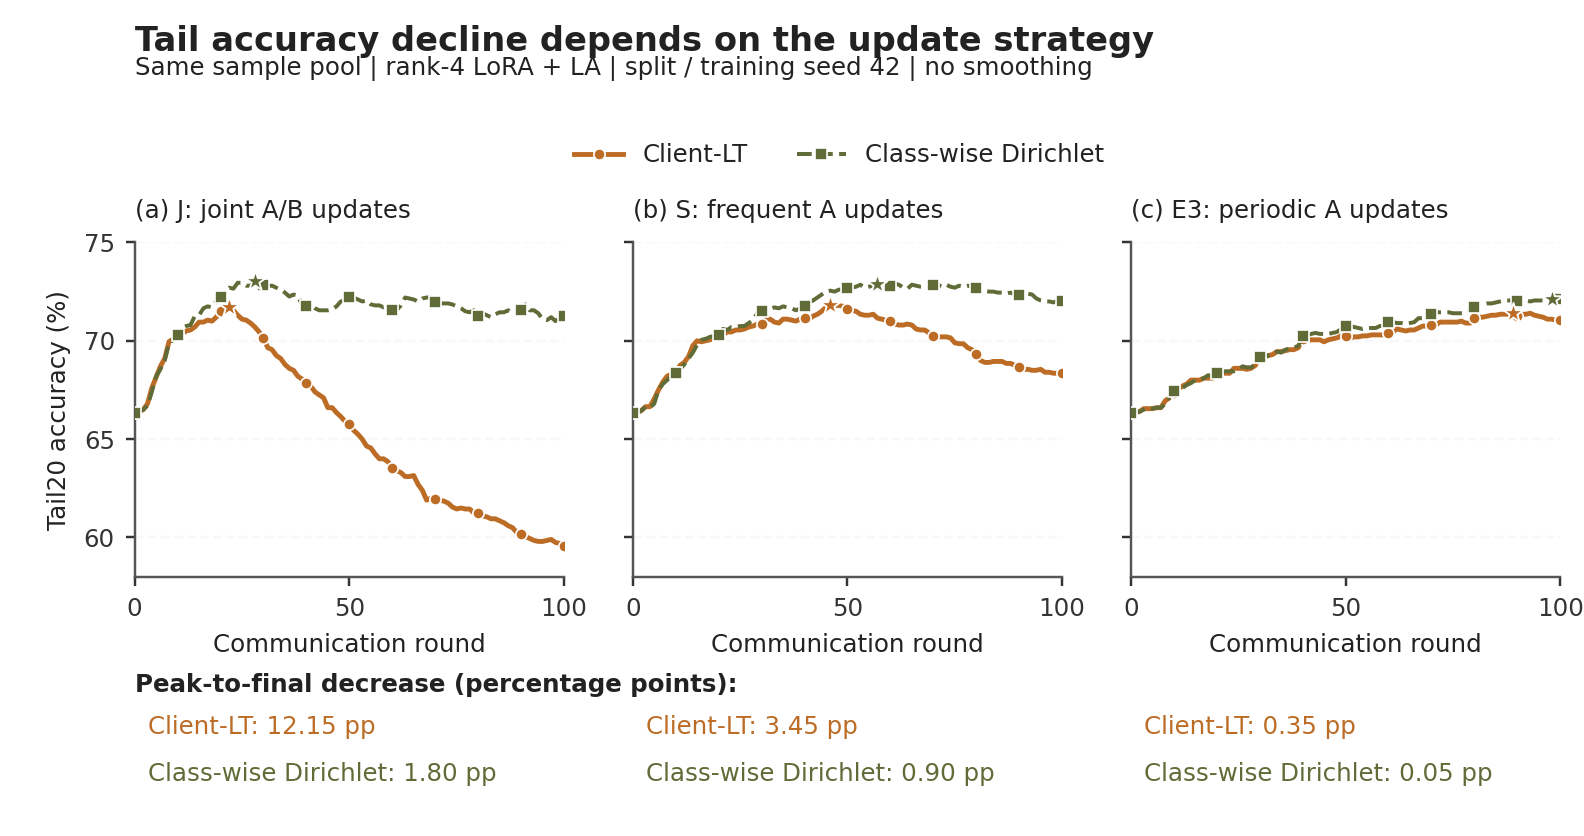
\includegraphics[width=0.95\linewidth]{retention_comparison.png}\end{center}

{\small\noindent 图 2. 三种参数更新策略下的尾部类别准确率。曲线来自训练种子与划分种子均为 42 的 rank-4 实验。J、S、E3 的更新日程见正文；J 为训练策略名称，方法中的 joint 表示聚合权重。\par}

为进一步考察客户端分配，我们构造固定边际的 matched 对照，同时保持每类样本总量 $n_c$ 和每个客户端样本总量 $n_k$ 不变。在 J 策略中，matched 的尾部类别准确率从峰值 73.20\% 下降至 72.80\%；在 S 策略中，从 72.75\% 下降至 72.10\%。与对应的 Client-LT 轨迹相比，这一结果表明，即使类别数量和客户端容量相同，类别样本由哪些客户端共同持有，仍是理解尾部类别保持表现的重要实验条件。


\subsection*{3.3 从样本所在位置到更新的有效支持}

为理解客户端更新如何作用于尾部类别，我们在一组 rank-2 LoRA 诊断实验中，沿实际全局更新路径分解类别预测分数的变化。诊断分数取正确类别 logit 与其他类别 logits 的 logsumexp 之差，并在该类别分析样本上求平均。贡献按客户端是否含有目标类别样本，以及作用方向为正或负进行分组。


对第 11—100 轮的贡献进行时间累计并在尾部 20 类上平均后，含目标类别样本客户端的正向贡献，在 matched 与 Client-LT 中分别为 14.553 和 6.874；全部客户端的正向贡献分别为 29.200 和 24.516。与此同时，不含目标类别样本客户端的正向贡献分别为 14.646 和 17.642，其负向贡献分别为 28.353 和 25.612。这些量以诊断分数变化计量，反映了持续训练中正向支持的来源及其变化。


上述观察给出两个相连的方法切入点。第一，维护某个类别的已有能力，需要关注哪些客户端更新仍能持续改善它的预测，以及这些正向作用是否集中于少数来源。第二，不含目标类别样本的客户端也可能提供有益更新，因此利用客户端知识时应进一步考虑更新对目标类别的作用。由此，我们分别设计基于来源响应的知识保持和基于反馈的更新组合，使已有能力的维护与额外学习支持围绕同一个全局模型展开。


\section*{4. 方法}

\subsection*{4.1 整体框架}

我们在冻结的 CLIP 主干上使用 LoRA 进行视觉适配。第 $\ell$ 个适配层的权重为


\begin{center}\begin{adjustbox}{max width=\linewidth}$\displaystyle W_\ell=W_{0\ell}+\gamma_\ell B_\ell A_\ell,$\end{adjustbox}\end{center}

其中，$W_{0\ell}$ 为预训练权重，$A_\ell$ 和 $B_\ell$ 为可训练低秩因子，$\gamma_\ell$ 为缩放系数。每轮从共同全局模型出发，先固定因子 $A_\ell$ 训练 $B_\ell$，再在开放的轮次固定共同的 $B_\ell$ 训练 $A_\ell$。本文将两个算法组件分别称为方法 A 和方法 B：方法 A 在因子 $A_\ell$ 的普通更新后实施知识保持修正，方法 B 在因子 $B_\ell$ 的普通聚合后构造补充更新。


整体框架使用三类信息。客户端类别计数用于确定普通聚合权重；当前客户端更新与本地预测间隔用于确定保持优先级和改善目标；历史预测间隔用于记录已经持续获得的能力。方法 B 进一步利用本地分类反馈，将当轮已有客户端更新组合成共享残差。所有反馈图像保留在所属客户端，服务器依据上传的反馈量与梯度完成协调。


\subsection*{4.2 基于类别分布的 joint 聚合}

Client-LT 中，集中持有尾部类别样本的客户端可能具有较小的总数据量。为在普通聚合中考虑这一分布，我们根据各客户端的类别组成共同求解聚合权重。记客户端样本量权重为 $\pi_j=n_j/N$，本地类别比例为 $P_{jc}=n_{jc}/n_j$，其中 $N=\sum_jn_j$。权重 $w$ 所对应的类别分布代理为 $P^\top w$；当 $w=\pi$ 时，该代理等于全局训练类别频率。


我们以均匀类别分布 $u_c=1/C$ 为目标，并用相对样本量权重的偏离控制聚合调整幅度：


\begin{center}\begin{adjustbox}{max width=\linewidth}$\displaystyle w^*=\arg\min_{w\geq0,\,\mathbf1^\top w=1}
D_{\mathrm{KL}}\!\left(u\,\|\,P^\top w\right)
+\frac{\lambda_{\mathrm{agg}}}{2}
\sum_{j=1}^{K}\frac{(w_j-\pi_j)^2}{\pi_j}.$\end{adjustbox}\end{center}

第一项使各客户端类别分布的加权组合接近目标分布，第二项保留客户端数据量提供的参考。对于固定数据划分与全参与训练，服务器在训练前求解一次权重，并将同一组 $w^*$ 用于普通 $B_\ell$ 聚合和普通 $A_\ell$ 提案聚合。本文取 $\lambda_{\mathrm{agg}}=0.1$。


joint 聚合提供类别分布层面的调整。随着模型不断更新，同一客户端对某个类别的作用也可能改变；后续知识保持与知识迁移因此进一步使用模型当前产生的反馈。


\subsection*{4.3 方法 A：来源感知的知识保持}

方法 A 的目标是在允许模型继续适配的同时，维护那些有效支持较为集中的类别能力。为此，我们先衡量客户端更新对预测的作用，再确定保持权重和目标，最后修正常规聚合结果。


\paragraph{预测间隔与客户端更新响应}

对每个非空客户端—类别组合 $q=(k,c)$，从本地训练集中固定选取至多 8 张图像，组成反馈样本集 $\mathcal W_q$。采用原图和水平翻转两个确定性视图，以正确类别与最强竞争类别的余弦分数差定义平均预测间隔：


\begin{center}\begin{adjustbox}{max width=\linewidth}$\displaystyle F_{qv}(A)=\frac{1}{|\mathcal W_q|}
\sum_{x\in\mathcal W_q}
\left[s_c(v(x);A,\bar B)
-\max_{c'\ne c}s_{c'}(v(x);A,\bar B)\right].$\end{adjustbox}\end{center}

其中，$A$ 表示本阶段全部可训练的 $A_\ell$ 因子，$\bar B$ 表示该阶段共同固定的 $B_\ell$ 因子，$v$ 为视图。预测间隔直接刻画正确类别相对竞争类别的分数优势；本地分类训练仍使用 logit adjustment，保持反馈则采用原始余弦分数。


令本阶段共同起点为 $A_t$，客户端 $j$ 的更新为 $\Delta A_j=A_j^{\mathrm{loc}}-A_t$，常规聚合提案为


\begin{center}\begin{adjustbox}{max width=\linewidth}$\displaystyle A_t^{\mathrm{ord}}=A_t+\sum_{j=1}^{K}w_j^*\Delta A_j.$\end{adjustbox}\end{center}

通过预测间隔梯度与更新的内积，得到客户端更新的局部响应：


\begin{center}\begin{adjustbox}{max width=\linewidth}$\displaystyle r_{qvj}=\left\langle\nabla_A F_{qv}(A_t),\Delta A_j\right\rangle.$\end{adjustbox}\end{center}

当两个视图上的响应均超过 $10^{-6}$ 时，取两者较小值作为 $a_{qj}$，否则令 $a_{qj}=0$。这一规则使正向支持同时满足两个视图的预测要求，并保留其响应强度。


\paragraph{有效支持的集中程度}

具有相同标签样本数的两个客户端—类别组合，可能从不同数量、不同强度的客户端更新中获得帮助。我们据正向响应计算有效客户端数：


\begin{center}\begin{adjustbox}{max width=\linewidth}$\displaystyle N_q^{\mathrm{eff}}
=\frac{\left(\sum_j a_{qj}\right)^2}{\sum_j a_{qj}^2},
\qquad
\rho_q=\frac{1}{N_q^{\mathrm{eff}}},
\qquad
\omega_q=\frac{\rho_q}{\sum_{q'\in\mathcal Q_{\mathrm{active}}}\rho_{q'}}.$\end{adjustbox}\end{center}

正向作用集中于较少客户端时，$N_q^{\mathrm{eff}}$ 较小，对应的保持权重较高；正向作用分散于更多客户端时，权重相应降低。这将保持约束分配给有效支持更集中的类别功能。若当前没有正向响应，则沿用该组合此前的 $\rho_q$，其初值为 $1/K$。$\mathcal Q_{\mathrm{active}}$ 包含具有当前目标或有效历史目标的组合。


\paragraph{当前目标与历史预测间隔}

保持目标需要同时反映当前可获得的改善和此前持续达到的水平。对于存在正向响应的组合，令 $u_q$ 为正向响应的均值，构造当前目标：


\begin{center}\begin{adjustbox}{max width=\linewidth}$\displaystyle u_q=\frac{\sum_j a_{qj}}{|\{j:a_{qj}>0\}|},
\qquad
T_{qv}^{\mathrm{cur}}=\min\left(2,F_{qv}(A_t)+0.5u_q\right).$\end{adjustbox}\end{center}

当前目标将更新中可利用的正向作用转化为预测间隔的改善要求。为使这一要求在后续能力回落时仍保留时间参照，我们按连续五轮、互不重叠的区间记录每轮最终全局模型的预测间隔。每个区间取五轮、两个视图上的最低值；当它比已有有效记录至少高出 0.001 时，更新历史值 $H_q$。首次登记以前，以初始模型的双视图最低预测间隔作为判断改善的参照。


当当前目标与历史记录同时存在时，保持目标为


\begin{center}\begin{adjustbox}{max width=\linewidth}$\displaystyle T_{qv}=\max\left(T_{qv}^{\mathrm{cur}},H_q\right).$\end{adjustbox}\end{center}

仅有其中一种目标时使用该目标，两者均不存在时该组合不参与保持损失。新登记的历史值从下一轮开始使用。由此，当前目标推动已有更新所支持的改善，历史目标则使已经持续达到的预测间隔继续参与后续适配。


\paragraph{兼顾知识保持与分类学习的更新修正}

我们在普通聚合提案附近优化保持目标。令 $R_t=\sqrt{K^{-1}\sum_j\|\Delta A_j\|^2}$ 表示客户端更新的均方根幅度，以 $A(z)=A_t^{\mathrm{ord}}+R_tz$ 参数化修正模型，并约束 $\|z\|\leq1$。知识保持损失为


\begin{center}\begin{adjustbox}{max width=\linewidth}$\displaystyle \mathcal L_{\mathrm{keep}}(z)
=\sum_{q\in\mathcal Q_{\mathrm{active}}}
\frac{\omega_q}{4}\sum_{v=1}^{2}
\left[\frac{T_{qv}-F_{qv}(A(z))}{\sigma_{qv}}\right]_+^2,
\qquad
\sigma_{qv}=\max\left(10^{-3},R_t\|\nabla_A F_{qv}(A_t)\|\right),$\end{adjustbox}\end{center}

其中 $[x]_+=\max(x,0)$。损失仅作用于尚未达到目标的预测间隔，尺度 $\sigma_{qv}$ 结合更新幅度与局部敏感度对不同组合进行归一化。


为协调保持修正与分类学习，记 $\widehat L(A)$ 为反馈样本上的 LA 分类损失，按客户端样本占比 $\pi_k$ 及其本地类别频率加权。我们对分类损失相对普通提案的增加施加软惩罚：


\begin{center}\begin{adjustbox}{max width=\linewidth}$\displaystyle \mathcal R_{\mathrm{cls}}(z)
=\frac12\left[
\frac{\widehat L(A(z))-\widehat L(A_t^{\mathrm{ord}})}{\xi_t}
\right]_+^2,
\qquad
\xi_t=\max\left(10^{-3},R_t\|\nabla_A\widehat L(A_t^{\mathrm{ord}})\|\right).$\end{adjustbox}\end{center}

最终求解


\begin{center}\begin{adjustbox}{max width=\linewidth}$\displaystyle \min_{\|z\|\leq1}
\frac12\|z\|^2
+\lambda_F\mathcal L_{\mathrm{keep}}(z)
+\mu_{\mathrm{cls}}\mathcal R_{\mathrm{cls}}(z).$\end{adjustbox}\end{center}

三项分别控制偏离普通更新的幅度、已有预测间隔的损失，以及分类训练目标的恶化。本文取 $\lambda_F=10$、$\mu_{\mathrm{cls}}=1$，从 $z=0$ 开始，以步长 0.1 执行三次投影梯度更新。每次修正中，目标、权重和归一化尺度保持固定。得到的因子 $A$ 与本轮共同因子 $B$ 一起构成本轮全局模型。


\subsection*{4.4 方法 B：反馈驱动的跨客户端知识迁移}

知识保持为已经获得的能力提供约束，客户端更新组合则提供进一步利用共享训练信息的途径。方法 B 保留普通 $B_\ell$ 训练阶段产生的更新 $\Delta B_{j\ell}$，并依据目标类别反馈学习这些更新如何组成一个有用的共享补充。


我们先在普通聚合模型上测试候选更新。对于客户端 $k$ 持有、而客户端 $j\ne k$ 不含有的尾部类别，加入 $0.1\Delta B_j$ 后计算本地 LA 分类损失。若至少一个此类类别的损失下降，则将 $j$ 加入客户端 $k$ 的候选集合，再对这些集合取并集，得到来源集合 $\mathcal D$。随后对并集内的更新统一进行反馈优化。


对每个来源客户端 $j$ 和 LoRA 层 $\ell$，设置独立的 $r\times r$ 组合矩阵 $C_{j\ell}$。补充更新与候选全局因子为


\begin{center}\begin{adjustbox}{max width=\linewidth}$\displaystyle R_\ell(C)=\frac{1}{|\mathcal D|}
\sum_{j\in\mathcal D}\Delta B_{j\ell}C_{j\ell},
\qquad
B_\ell(C)=\bar B_\ell+R_\ell(C),$\end{adjustbox}\end{center}

其中，$\bar B_\ell$ 为当前轮 joint 聚合后的普通因子。矩阵 $C_{j\ell}$ 在低秩维度上调整各来源更新，再将其组合到同一个全局模型中。组合参数在所有反馈客户端之间共享，分别对应各个来源和各个适配层。


记 $\mathcal R$ 为实际含有尾部类别样本的客户端集合。对同时含有尾部与非尾部样本的客户端，分别轮换采样两组图像，计算


\begin{center}\begin{adjustbox}{max width=\linewidth}$\displaystyle L_k(C)=\eta_T L_{k,T}(C)+(1-\eta_T)L_{k,N}(C),
\qquad \eta_T=0.35.$\end{adjustbox}\end{center}

仅含尾部样本的客户端使用 $L_{k,T}(C)$。各反馈客户端等权参与组合矩阵的优化：


\begin{center}\begin{adjustbox}{max width=\linewidth}$\displaystyle \mathcal J_B(C)=\frac{1}{|\mathcal R|}\sum_{k\in\mathcal R}L_k(C)
+\frac{\lambda_C}{|\mathcal D|L}
\sum_{j\in\mathcal D}\sum_{\ell=1}^{L}\|C_{j\ell}\|_F^2,
\qquad \lambda_C=0.001.$\end{adjustbox}\end{center}

其中，$L$ 为 LoRA 适配层数。尾部反馈引导补充更新服务于稀缺类别，非尾部反馈使优化同时考虑其他类别的分类表现，矩阵正则控制组合强度。每次执行时将 $C$ 初始化为零，固定普通聚合因子与客户端更新，采用学习率为 0.3 的 Adam 优化两步，然后将最终残差一次性合并到 $B_\ell$。


这一补充直接复用当轮客户端更新，并在合并后继续原有联邦训练。推理阶段使用一个全局 LoRA 模型。


\subsection*{4.5 完整训练过程}

训练开始前，服务器收集客户端类别计数并求解 joint 权重。每轮首先固定 $A_\ell$，由所有客户端训练 $B_\ell$ 三个本地 epoch，然后使用 $w^*$ 聚合。在第 30、40、……、100 轮，执行方法 B，以普通聚合后的模型为起点形成共享补充更新。


在第 1—90 轮，所有客户端进一步固定更新后的共同 $B_\ell$，训练 $A_\ell$ 一个本地 epoch。服务器形成 joint 聚合提案，利用客户端反馈执行方法 A 的三步修正，再提交本轮全局模型并更新历史记录。第 91—100 轮继续 $B_\ell$ 的训练和相应的补充更新。整个过程使类别分布、当前更新响应和历史能力分别在聚合、学习与保持中发挥作用。


\section*{5. 实验}

\subsection*{5.1 实验设置}

我们在 CIFAR-100-LT 的固定 Client-LT 划分上开展方法开发与机制分析。全局不平衡因子为 100，训练集包含 10,847 张图像，测试集每类 100 张。客户端数量为 30，每轮全部参与，共训练 100 轮。划分采用 $q_T=0.1$、$\lambda_T=0.75$ 和组内 Dirichlet 参数 $\alpha_T=0.5$，划分种子为 42。按照训练样本数量排序，前 20 类、中间 60 类和最后 20 类分别记为 Head20、Middle60 和 Tail20。


本文方法使用 CLIP ViT-B/16，在视觉编码器最后三个 block 的 q/v 投影中加入 rank-4 LoRA，共六个适配层，缩放系数为 $1/\sqrt r$，采用 FP32 训练。本地训练批大小为 32，使用 SGD，学习率为 0.001，动量为 0.9。普通 $B_\ell$ 训练的权重衰减为 0.0005，$A_\ell$ 训练的权重衰减为零。LA 使用全局训练类别频率，系数为 1；方法 A 和方法 B 的配置见第 4 节。


分类性能统一报告第 81—100 轮最终全局模型的准确率均值，并同时保留 Overall、Head20、Middle60 和 Tail20。保持分析包括峰值至末轮的准确率回落，以及从共同检查点继续训练后的正确$\rightarrow$错误、错误$\rightarrow$正确样本数。主配置比较采用训练种子 42；知识保持和更新组合的模块分析使用原样本量聚合协议下种子 42、3407 的配对运行。


对比方法包括普通 FedAvg-LoRA、加入全局 LA 的 FedAvg-LoRA、CAPT、FedPuReL、FedNTD、FedLF、FedYoYo、FedReLa，以及 RoLoRA、FedSVD 和 LoRA-A$^2$。比较采用共享 CLIP 骨干的实验实现：CAPT 使用固定聚合版本，FedPuReL 使用全局阶段，FedSVD 使用非 DP 版本；FedNTD、FedLF、FedYoYo、FedReLa 及联邦 LoRA 方法采用表中注明的 CLIP-LoRA 适配。不同方法的本地训练与额外反馈计算按各自流程执行。


\subsection*{5.2 完整配置的分类性能}

表 1 汇总共享 CLIP 设置下的开发实验。本文完整配置的 Tail20 为 72.6325\%，Overall 为 70.4700\%。在该表的已测配置中，本文方法取得最高的尾部类别准确率，FedAvg-LoRA＋LA 则取得最高的整体准确率。二者分别为 72.6325\%/60.3575\% 的 Tail20 和 70.4700\%/71.1845\% 的 Overall，表明训练目标与更新组织方式对类别组之间的性能分配具有明显影响。


\noindent\begin{minipage}{\linewidth}{\small 表 1. CIFAR-100-LT、Client-LT 上的配置比较。数值为训练种子 42、第 81—100 轮准确率均值，单位为 \%。各行使用其注明的算法版本与训练流程。\par}\medskip

\noindent{\small\begin{tabularx}{\linewidth}{p{0.40\linewidth}*{4}{>{\raggedleft\arraybackslash}X}}\toprule

方法及实验版本 & Overall & Head20 & Middle60 & Tail20 \\ \midrule

FedAvg-LoRA，联合训练、CE & 64.5325 & 85.6300 & 66.9625 & 36.1450 \\

FedAvg-LoRA＋全局 LA，联合训练 & 71.1845 & 78.4525 & 72.3708 & 60.3575 \\

CAPT，固定聚合版本 & 66.8210 & 79.2675 & 61.2208 & 71.1750 \\

FedPuReL-Global，CLIP-LoRA 适配 & 65.7625 & 70.5475 & 64.1892 & 65.6975 \\

FedNTD，CLIP-LoRA 适配 & 64.1465 & 86.1150 & 65.7792 & 37.2800 \\

FedLF，CLIP-LoRA 适配 & 67.7295 & 77.3550 & 70.5433 & 49.6625 \\

FedYoYo，CLIP-LoRA 适配 & 64.4635 & 67.8950 & 67.6892 & 51.3550 \\

FedAvg-LoRA＋FedReLa，CE 训练与一次重标记 & 65.6160 & 83.2900 & 67.9550 & 40.9250 \\

RoLoRA，CLIP 交替因子适配 & 63.2170 & 85.6725 & 64.6675 & 36.4100 \\

FedSVD，非 DP 的 CLIP-LoRA 适配 & 67.2670 & 82.9175 & 63.6842 & 62.3650 \\

LoRA-A$^2$，全局 rank-4 的 CLIP 适配 & 65.0985 & 85.6950 & 67.2892 & 37.9300 \\

本文方法，joint＋A＋B & 70.4700 & 73.9950 & 68.5742 & 72.6325 \\

\bottomrule\end{tabularx}}\end{minipage}\par

与 CAPT 的已测配置相比，本文方法的 Tail20 和 Overall 分别高出 1.4575 和 3.6490 个百分点。进一步观察普通交替训练的两种聚合配置：joint 使用第 4.2 节的权重，TailRW16 则按 $(n_j+16n_{j,T})/(N+16N_T)$ 加权，其中 $n_{j,T}$ 和 $N_T$ 分别为本地与全局尾部样本数。两种配置的 Tail20/Overall 分别为 71.7075\%/70.8655\% 和 72.2775\%/70.9115\%。本文完整配置在这组配置比较中具有更高的尾部类别准确率，同时整体准确率较低。后续模块分析进一步考察，保持目标与更新组合分别改变了哪些预测行为。


\subsection*{5.3 来源权重与历史目标的作用}

我们在按样本量聚合的协议下开展配对模块实验，固定各组的因子更新频率。普通交替训练执行相同的本地适配；A-flat 将方法 A 的保持损失权重设为均匀，保留当前目标与历史目标；A-current 使用来源感知权重，仅使用当前目标。表 2 同时列出方法 B 及直接校准对照，以呈现保持与补充更新的组合效果。


\noindent\begin{minipage}{\linewidth}{\small 表 2. 原样本量聚合下的两个随机种子的模块实验。数值为第 81—100 轮准确率均值，单位为 \%。各组采用相同的普通因子训练日程。\par}\medskip

\noindent{\small\begin{tabularx}{\linewidth}{p{0.40\linewidth}*{4}{>{\raggedleft\arraybackslash}X}}\toprule

配置 & Overall，42 & Tail20，42 & Overall，3407 & Tail20，3407 \\ \midrule

普通交替训练 & 70.9100 & 68.6625 & 70.9295 & 69.0775 \\

A-flat，均匀保持权重 & 70.7125 & 70.0550 & 70.7840 & 70.5325 \\

A-current，仅当前目标 & 70.8670 & 68.9350 & 70.8730 & 69.3225 \\

方法 A & 70.6330 & 70.9350 & 70.4770 & 71.0900 \\

方法 A＋方法 B & 70.6965 & 71.1575 & 70.5115 & 71.2200 \\

方法 A＋直接校准 & 70.6695 & 71.2575 & 70.4295 & 71.3075 \\

\bottomrule\end{tabularx}}\end{minipage}\par

来源感知权重在两个训练种子中均带来额外的尾部类别收益。方法 A 相对 A-flat 的 Tail20 分别提高 0.8800 和 0.5575 个百分点，说明正向作用的来源分布可以为保持约束的分配提供有效信息。该设计将有限的修正能力优先分配给有效支持较集中的客户端—类别组合。


历史目标提供了更明显的保持收益。方法 A 相对 A-current 的 Tail20 分别提高 2.0000 和 1.7675 个百分点；尾部类别峰值至末轮的回落由 3.35/2.60 缩小为 1.00/0.50 个百分点。当前目标根据当前模型与更新响应形成，历史记录则保存此前持续达到的预测间隔。两者的配合使保持要求同时具有当前方向与跨轮参照。


完整方法 A 相对普通交替训练的 Tail20 分别提高 2.2725 和 2.0125 个百分点，Overall 分别降低 0.2770 和 0.4525 个百分点。这一结果呈现了方法的直接作用：增强尾部类别能力的保持，同时改变全局模型在不同类别之间的适配分配。


\subsection*{5.4 尾部类别收益对应的样本变化}

为进一步观察能力保持，我们从方法 A 在第 60 和第 80 轮的同一模型出发，分别继续训练五轮。比较完整方法 A、普通更新，以及保持普通更新方向但匹配修正后更新幅度的对照。表 3 分别统计尾部测试样本中由正确变错和由错误变对的数量。


\noindent\begin{minipage}{\linewidth}{\small 表 3. 同起点五轮继续训练后的 Tail20 预测变化。尾部测试样本共 2,000 张；第 60、80 轮起点准确率分别为 71.55\% 和 71.25\%。\par}\medskip

\noindent{\small\begin{tabularx}{\linewidth}{X*{4}{>{\raggedleft\arraybackslash}X}}\toprule

起点轮次 & 后续更新 & 正确$\rightarrow$错误，张 & 错误$\rightarrow$正确，张 & 五轮后 Tail20，\% \\ \midrule

60 & 普通更新 & 8 & 3 & 71.30 \\

60 & 幅度匹配 & 5 & 3 & 71.45 \\

60 & 方法 A & 2 & 2 & 71.55 \\

80 & 普通更新 & 15 & 3 & 70.65 \\

80 & 幅度匹配 & 8 & 1 & 70.90 \\

80 & 方法 A & 6 & 1 & 71.00 \\

\bottomrule\end{tabularx}}\end{minipage}\par

在两个起点上，方法 A 都减少了已经正确分类样本的丢失。相对普通更新，正确$\rightarrow$错误的样本数分别从 8 降至 2、从 15 降至 6；相对幅度匹配更新，也进一步减少。与此同时，方法 A 在两个起点分别新增 2 和 1 张正确分类样本，普通更新均新增 3 张。这些变化将平均准确率分解为保持与学习两个过程：当前收益主要伴随着更少的已有正确预测丢失，而新获得的正确预测数量也受到更新修正的影响。


\subsection*{5.5 客户端更新组合的补充作用}

在表 2 的两个随机种子的实验中，方法 B 加入方法 A 后，Tail20 分别提高 0.2225 和 0.1300 个百分点，Overall 分别提高 0.0635 和 0.0345 个百分点。方法 B 在固定普通聚合结果的基础上优化组合矩阵，使已有客户端更新进一步响应尾部与非尾部类别反馈。


我们进一步比较直接校准：在 $B_\ell$ 的全坐标残差上优化分类损失，使用相同的反馈样本、分组损失权重和优化步数，并在每步匹配两种方法对应权重增量的范数。方法 B 的 Tail20 比直接校准分别低 0.1000 和 0.0875 个百分点，Overall 分别高 0.0270 和 0.0820 个百分点。两种参数化取得了不同的类别性能分配，客户端更新组合在当前实验中提供了较高的整体准确率，而直接校准获得了略高的尾部类别准确率。


在完整 joint＋A＋B 配置的八次方法 B 执行中，候选来源并集均包含全部 30 个客户端。因此，该配置实际在全部来源更新上学习各自的矩阵变换，反馈优化决定了这些更新的组合方式。这一实现将跨客户端知识迁移具体落实为对已有更新的重新利用，并通过共享残差服务于最终全局模型。


\subsection*{5.6 训练开销与学习保持的取舍}

本文方法增加的训练开销来自额外因子适配、保持反馈和组合优化。在当前 Client-LT 划分中，普通 $B_\ell$ 训练执行 105,600 个本地优化步，前 90 轮的 $A_\ell$ 适配增加 31,680 步。方法 A 另外执行 270 次投影修正；方法 B 在八个轮次中共执行 16 次组合矩阵优化。joint 权重只在训练前求解一次。


反馈计算也是通信成本的主要来源。在原样本量聚合的两个随机种子的模块实验中，方法 A 的额外模拟上行和下行通信量分别约为 1.23 GB 和 6.80 GB；方法 B 分别约为 4.07 MB 和 406.40 MB。当前六个适配层、rank-4、30 个来源客户端对应 2,880 个组合参数，补充更新合并后沿用原有全局 LoRA 结构。因而，方法的主要成本发生在训练阶段的反馈与修正。


分类结果和样本变化共同表明，维护历史能力会改变后续适配的取向。来源感知权重与历史目标增强了尾部类别的保持，但整体准确率和新学习样本数也呈现出相应取舍。进一步降低反馈成本，并使保持强度更贴合各阶段的学习需求，是这一方法值得继续研究的方向。


\section*{6. 结论}

本文研究尾部类别样本集中于少数客户端时，全局模型如何在持续联邦训练中保持已有分类能力。通过相同全局样本池的划分比较、固定边际对照和客户端更新分析，我们将类别样本数量、客户端分布与训练中的有效支持联系起来。基于这一视角，本文在类别分布感知聚合之上，以来源响应和历史预测间隔指导知识保持，并利用本地反馈学习客户端更新的共享组合。CIFAR-100-LT 上的配置比较和模块实验呈现出尾部类别的保持收益，也揭示了保持、继续学习与训练成本之间的关系。让少数客户端提供的样本持续支撑全局模型的分类能力，为联邦长尾适配提供了一个明确的优化目标。


\section*{参考文献}

{\small\noindent [1] Brendan McMahan, Eider Moore, Daniel Ramage, Seth Hampson, Blaise Agüera y Arcas. \href{https://proceedings.mlr.press/v54/mcmahan17a.html}{Communication-Efficient Learning of Deep Networks from Decentralized Data}. AISTATS, 2017.\par}

{\small\noindent [2] Alec Radford, Jong Wook Kim, Chris Hallacy, et al. \href{https://proceedings.mlr.press/v139/radford21a.html}{Learning Transferable Visual Models From Natural Language Supervision}. ICML, 2021.\par}

{\small\noindent [3] Jiang-Xin Shi, Tong Wei, Zhi Zhou, Jie-Jing Shao, Xin-Yan Han, Yu-Feng Li. \href{https://proceedings.mlr.press/v235/shi24g.html}{Long-Tail Learning with Foundation Model: Heavy Fine-Tuning Hurts}. ICML, 2024.\par}

{\small\noindent [4] Shihao Hou, Xinyi Shang, Shreyank N Gowda, et al. \href{https://arxiv.org/abs/2503.06993}{CAPT: Class-Aware Prompt Tuning for Federated Long-Tailed Learning with Vision-Language Model}. arXiv:2503.06993, 2025.\par}

{\small\noindent [5] Shihao Hou, Chikai Shang, Zhiheng Yang, et al. \href{https://arxiv.org/abs/2605.02247}{Fine-Tuning Impairs the Balancedness of Foundation Models in Long-tailed Personalized Federated Learning}. CVPR, 2026.\par}

{\small\noindent [6] Gihun Lee, Minchan Jeong, Yongjin Shin, Sangmin Bae, Se-Young Yun. \href{https://proceedings.neurips.cc/paper_files/paper/2022/hash/fadec8f2e65f181d777507d1df69b92f-Abstract-Conference.html}{Preservation of the Global Knowledge by Not-True Distillation in Federated Learning}. NeurIPS, 2022.\par}

{\small\noindent [7] Youbang Sun, Zitao Li, Yaliang Li, Bolin Ding. \href{https://proceedings.iclr.cc/paper_files/paper/2024/hash/4e243e95c913b367775d71d7182b99d9-Abstract-Conference.html}{Improving LoRA in Privacy-preserving Federated Learning}. ICLR, 2024.\par}

{\small\noindent [8] Shuangyi Chen, Yuanxin Guo, Yue Ju, Harik Dalal, Zhongwen Zhu, Ashish Khisti. \href{https://arxiv.org/abs/2502.01755}{Robust Federated Finetuning of LLMs via Alternating Optimization of LoRA}. NeurIPS, 2025.\par}

{\small\noindent [9] Aditya Krishna Menon, Sadeep Jayasumana, Ankit Singh Rawat, Himanshu Jain, Andreas Veit, Sanjiv Kumar. \href{https://openreview.net/pdf?id=37nvvqkCo5}{Long-tail learning via logit adjustment}. ICLR, 2021.\par}

{\small\noindent [10] Xiuhua Lu, Peng Li, Xuefeng Jiang. \href{https://proceedings.mlr.press/v260/lu25a.html}{FedLF: Adaptive Logit Adjustment and Feature Optimization in Federated Long-Tailed Learning}. Proceedings of the 16th Asian Conference on Machine Learning, PMLR 260, 2025.\par}

{\small\noindent [11] Shanshan Yan, Zexi Li, Chao Wu, et al. \href{https://openaccess.thecvf.com/content/ICCV2025/html/Yan_You_Are_Your_Own_Best_Teacher_Achieving_Centralized-level_Performance_in_ICCV_2025_paper.html}{You Are Your Own Best Teacher: Achieving Centralized-level Performance in Federated Learning under Heterogeneous and Long-tailed Data}. ICCV, 2025.\par}

{\small\noindent [12] Guangzheng Hu, Patricia Menendez, Feng Liu, Mingming Gong, Guanghui Wang, Liuhua Peng. \href{https://proceedings.mlr.press/v306/hu26ao.html}{FedReLa: Imbalanced Federated Learning via Re-Labeling}. ICML, 2026.\par}

{\small\noindent [13] Mariya Toneva, Alessandro Sordoni, Remi Tachet des Combes, Adam Trischler, Yoshua Bengio, Geoffrey J. Gordon. \href{https://arxiv.org/abs/1812.05159}{An Empirical Study of Example Forgetting during Deep Neural Network Learning}. ICLR, 2019.\par}

{\small\noindent [14] Edward J. Hu, Yelong Shen, Phillip Wallis, et al. \href{https://arxiv.org/abs/2106.09685}{LoRA: Low-Rank Adaptation of Large Language Models}. arXiv:2106.09685, 2021.\par}

{\small\noindent [15] Seanie Lee, Sangwoo Park, Dong Bok Lee, et al. \href{https://arxiv.org/abs/2505.12805}{FedSVD: Adaptive Orthogonalization for Private Federated Learning with LoRA}. NeurIPS, 2025.\par}

{\small\noindent [16] Jabin Koo, Minwoo Jang, Jungseul Ok. \href{https://aclanthology.org/2025.acl-long.19/}{Towards Robust and Efficient Federated Low-Rank Adaptation with Heterogeneous Clients}. ACL, 2025.\par}

{\small\noindent [17] Zheng Wang, Xiaoliang Fan, Jianzhong Qi, Chenglu Wen, Cheng Wang, Rongshan Yu. \href{https://www.ijcai.org/proceedings/2021/223}{Federated Learning with Fair Averaging}. IJCAI, 2021.\par}

{\small\noindent [18] Nurbek Tastan, Samar Fares, Toluwani Aremu, Samuel Horváth, Karthik Nandakumar. \href{https://www.ijcai.org/proceedings/2024/554}{Redefining Contributions: Shapley-Driven Federated Learning}. IJCAI, 2024.\par}

{\small\noindent [19] Michael Zhang, Karan Sapra, Sanja Fidler, Serena Yeung, Jose M. Alvarez. \href{https://arxiv.org/abs/2012.08565}{Personalized Federated Learning with First Order Model Optimization}. ICLR, 2021.\par}

{\small\noindent [20] Alex Krizhevsky. \href{https://www.cs.toronto.edu/~kriz/learning-features-2009-TR.pdf}{Learning Multiple Layers of Features from Tiny Images}. University of Toronto, Technical Report, 2009.\par}

\end{document}